\documentclass[12pt]{article}
\usepackage{amsmath}
\usepackage{jheppub}
\usepackage{marginnote,xparse,changepage,caption}

\newcommand{\IGNORE}[1]{}
\newcommand{\be}{\begin{equation}}
\newcommand{\ee}{\end{equation}}
\newcommand{\bea}{\begin{aligned}}
\newcommand{\eea}{\end{aligned}}
\newcommand{\mb}[1]{\marginnote{\color{red}{\small MB:\,#1}}}
\renewcommand{\ij}[1]{\marginnote{\color{red}{\small IJ:\,#1}}}
\renewcommand{\ss}[1]{\marginnote{\color{red}{\small SS:\,#1}}}
\newcommand{\ibar}{{\overline{\emph\i}}}
\newcommand{\jbar}{{\overline{\emph\j}}}

\title{Boundary terms in the action for Causal Sets}
 \author[a]{Michel Buck}
 \author[a,b]{\!, Fay Dowker}
 \author[a]{\!, Ian Jubb\,}
 \author[c]{and Sumati Surya}
\affiliation[a]{Theoretical Physics Group, Blackett Laboratory, Imperial College, London, SW7 2AZ, U.K.}
\affiliation[b]{Institute for Quantum Computing, University of Waterloo, ON, N2L 2Y5, Canada}
\affiliation[c]{Raman Research Institute, CV Raman Ave, Sadashivanagar, Bangalore 560080, India}

\abstract{ 
We propose a family of formulae for the boundary term in the action of a causal set that is well-approximated by a continuum manifold with spacelike boundary. %The boundary term is proportional to the difference in the number of elements immediately to future and the number of elements immediately to the past of the surface. 
We show that in the continuum limit one recovers the Gibbons-Hawking-York boundary term in the mean.
}

\begin{document}

\maketitle

\section{Introduction}

%[MB1: USEFUL QUOTE FROM RAFAEL: In the quantum theory, however, these boundary terms are important. They are essential in order that the quantum mechanical amplitudes satisfy the correct composition law and in order that these amplitudes have the correct classical limit. In a number of examples [5] they give a contribution to the partition function which is important for the agreement with calculations based on straightforward thermodynamics. In this note we shall derive the boundary terms in the action for the Regge calculus]

In furthering causal set theory it is crucial that we understand the kinematics of the theory. The action of a given causal set is a crucial piece of the kinematics that would be extremely useful to know and understand. Proposals for the action of a causal set are available \cite{Benincasa_Dowker:The_Scalar_Curvature_of_a_Causal_Set} and these hold analytically in some cases and numerically in many more.\mb{rephrase} These cases being when the causal set is embeddable in some existing spacetime. One can show that the action of the causal set then agrees with the Einstein-Hilbert action of the spacetime in some continuum limit. How this limiting procedure is carried out will be described in more detail below.

It is well known that the Einstein-Hilbert action is not the full story in the continuum. In the presence of spacetime boundaries the gravitational action must include a boundary term $S_{GHY}$, the Gibbons-Hawking-York action, in order to yield a well-defined variational principle~\cite{Gibbons_Hawking_Boundary}. The contributions of this term play an essential role in particular in the quantum theory. For instance, in the calculation of the black hole entropy via the Euclidean path-integral, it is the boundary terms that produce the answer $A/4l_p^2$ necessary for the unification of black hole mechanics with thermodynamics. To give another example, in Regge calculus boundary terms are necessary in order that the quantum mechanical amplitudes satisfy the correct composition law and that they have the correct classical limit~\cite{hartlesorkin}.\mb{is this true?}

We define a \textit{causal set} (or \textit{causet}) as a locally finite partial order. This means it is a pair $(\mathcal{C},\preceq)$ where $\mathcal{C}$ is the set of points and $\preceq$ is a partial order relation on $\mathcal{C}$ that has the following properties. It is (i) reflexive: $x\preceq x$, (ii) acyclic: $x\preceq y\preceq x \Rightarrow x=y$, and (iii) transitive: $x\preceq y\preceq z \Rightarrow x\preceq z$ for all points $x, y, z \in \mathcal{C}$. We define an inclusive order interval as the set $I(x,y)\equiv \lbrace z\in\mathcal{C}|x\preceq z\preceq y\rbrace$ for any $x, y\in\mathcal{C}$. The \textit{locally finite} condition is simply that the cardinality of any order interval is finite, that is $|I(x,y)|<\infty$. This condition ensures we are dealing with a discrete structure, as all the other properties of the relation would apply to an order relation between points on a continuous manifold.

In order to say we have a causal set analogue for a continuous expression we need a well defined procedure for relating the discrete theory to the continuum. This procedure, or tool, is called a \textit{Poisson sprinkling}, or just a \textit{sprinkling}. It is a Poisson process which provides a way to generate a causet from a $d$-dimensional Lorentzian manifold $(M,g)$ by selecting certain points in $M$ to be the elements of $\mathcal{C}$, with an order relation given by the causal order of the manifold. The number of points chosen in a region of spacetime volume, $V$, is a Poisson random variable. This means that the expected number of points in some region will be $\rho V$, where $\rho$ is the density of the sprinkling. The density is related to the discreteness scale, $l$, by $\rho=l^{-d}$ in $d$ spacetime dimensions. It is called a sprinkling as one can envisage the point selection process as a `sprinkling' of points into the manifold. If a causet, $\mathcal{C}$, can be generated with relatively high probability by a sprinkling into the manifold, $(M,g)$, then we say that the manifold is a good approximation for the causal set.

\section{The Claims}

Consider a sufficiently well-behaved $d$-dimensional spacetime $(M,g)$ and Cauchy surface $\Sigma$ in $M$. The causal past and future sets $M^\pm=J^\pm(\Sigma)$ form a partition of $M$ and $\partial M^\pm = \Sigma$. The Gibbons-Hawking-York boundary term for $M^\pm$ is in this case given by
\be\label{eq:GHYBT_in_continuum}
S_{GHY} = \mp \frac{1}{l_p^{d-2}}\int_{\Sigma} K d\Sigma
\ee
where $l_p$ is the rationalised Planck length and $K$ is the trace of the extrinsic curvature $K_{\mu\nu}=h_{\mu}^\rho h_\nu^\sigma \nabla_\rho n_\sigma$ of $\Sigma$ defined with future-pointing timelike unit normal $n_{\mu}=\partial_\mu S/\sqrt{g^{\mu\nu}\partial_\mu S\partial_\nu S}$. (We will work with a mostly plus convention for the metric, in which this translates into a past-pointing normal vector $n^{\mu}$).\mb{ok or more detail on conventions needed?}

Now observe that the integral in~\eqref{eq:GHYBT_in_continuum} can be thought of as the ``volume gradient'' across the surface $\Sigma$. More formally
\be\label{eq:normal_deriv_boundary}
\int K d\Sigma = \frac{\partial}{\partial n}\int d\Sigma,
\ee
where the right hand side is the derivative of the area $\int d\Sigma$ as each point of $\Sigma$ is moved an equal distance along the unit normal vector, $n^{\mu}$, which corresponds to the rate of change of the surface volume backwards in time, as $n^{\mu}$ is past-pointing. 
\mb{does the antichain analogy really stand?} 

We will define the causal set analogue of a spacelike hypersurface to be a particular partition of the set $\mathcal{C}$ into parts $\mathcal{C}^+$ and $\mathcal{C}^-$. For this partition to make sense as a spacelike hypersurface we require that no elements in $\mathcal{C}^+$ can precede any elements in $\mathcal{C}^-$. The reason for this condition is that if one could faithfully embed $\mathcal{C}$ in some manifold, $M$ ($\mathcal{C}$ can be generated via a sprinkling into $M$), then given a spacelike hypersurface, $\Sigma$, we can partition the causet into two bits, denoting the future(past) part as $\mathcal{C}^+$($\mathcal{C}^-$), which is made up of those elements sprinkled into $M^+$($M^-$). The causal relations between the two parts immediately satisfy our requirement for the partition to be spacelike. We will refer to a partition as spacelike if it abides by this condition, even if the causet is not embeddable in some manifold. Spacetime volume in the causal set is obtained simply by counting the number of elements, and hence the volume gradient intuitively corresponds to the difference in the number of ``immediate neighbours'' to the future and to the past of the spacelike partition. What does it mean to be immediate neighbours to a spacelike partition? For immediate neighbours to the past(future) of the partition we mean elements of $\mathcal{C}^-$($\mathcal{C}^+$) that have no elements to their future(past) in $\mathcal{C}^-$($\mathcal{C}^+$) (these elements being called \textit{maximal}(\textit{minimal})). We shall see that this intuitive idea for the boundary term indeed bears out. However, one does not need to know the maximal and minimal elements to calculate the boundary term. It can be found from any elements that lie reasonably close to the surface (in the time coordinate on $M$) but are not necessarily maximal or minimal. This will be made more precise below.

In the continuum the GHY term can be calculated for a spacelike hypersurface, $\Sigma$, that is either a future or past boundary of $M$. We wish to calculate the GHY term for future or past boundaries of causets, but there are a couple issues we must deal with. Firstly, if we can embed a causet $\mathcal{C}$ into $M$ then the boundary surface of $M$ will not induce a partition of $\mathcal{C}$ as it did previously (every element of $\mathcal{C}$ will lie in the bulk of $M$), thus our previous idea for the boundary term does not work any more. Secondly, what does it mean to say a bounding surface of a causet if it is not embeddable in some manifold? Previously if the causet was not embeddable we could still define the surface as a partition of the causet. We shall see that the first issue is not a problem, and we will show that the GHY term can be found for a future(past) boundary of a causet (that is embeddable in $M$) by taking a difference in the number of certain elements that lie close to the future(past) bounding surface of $M$. We state that calculating the GHY term this way must apply whether or not the causet is embeddable, but this runs us into the second issue above. For what boundary are we calculating our GHY term if the causet is not embeddable? We propose that spacelike future and past boundaries exist for all causets of finite cardinality. By definition these causets are finite in temporal extent, and so if they can be embedded in some manifold then that manifold can always have spacelike future and past boundaries. These future and past boundaries are abstract objects for which quantities such as the GHY term can be calculated for. They only have physical meaning when the causet is embeddable in some manifold with a future(past) spacelike boundary, denoted $\Sigma$, in which case the quantities we calculate for the abstract future(past) boundary will agree with those calculated for $\Sigma$ (calculated with the continuum definitions) in some continuum limit.

One can also use partitions of a causet to define the causal set analogues of timelike and null hypersurfaces. If the partition is such that an element of $\mathcal{C}^-$ precedes and element of $\mathcal{C}^+$ which again precedes and element of $\mathcal{C}^-$, then the partition corresponds to a timelike hypersurface. If we have a partition that satisfies the requirements for a spacelike partition, we can define a null partition as that which has the following restrictions. For every $x_0\in\mathcal{C}^+$ one can find a sequence of elements $x_0 \succeq x_1 \succeq ...\succeq x_n$ such that $x_n$ is preceded by nothing and all the $x_i \in \mathcal{C}^+$; and for every $x_0\in\mathcal{C}^-$ one can find a sequence of elements $x_0 \preceq x_1 \preceq ...\preceq x_n$ such that $x_n$ precedes nothing and all the $x_i \in \mathcal{C}^-$. There is also the possibility of a surface changing between spacelike, timelike and null at different parts. In this case the situation is a little more complicated in causal set terms, and one must restrict to a suitable subsets of points such that one of the definitions for the different types of surfaces holds true while the others fail. This subset of points, with its particular relations across the particular partition, then corresponds to a portion of the surface being either spacelike, timelike or null.

%This suggests a very simple analogy for a causal set with a ``spacelike hypersurface''. \mb{under construction} The analogy These unrelated elements are maximal in the sense that there exist no elements $y\in\mathcal{C}\setminus\mathcal{A}$ such that $x\preceq y$, $\forall x\in\mathcal{A}$. 

Let us define the operators $N_{\vphantom{i}max}^{(k)}\left[\mathcal{C} \right]$ and $N_{min}^{(k)}\left[\mathcal{C}^- \right]$ that, for a given causet, $\mathcal{C}$, return the number of $k$-next-to-maximal/minimal elements respectively. A $k$-next-to-maximal(minimal) element is one for which there are $k$ elements to its future(past). This means that the $0$-to-maximal(minimal) elements are the maximal(minimal) elements.


Given a causet, $\mathcal{C}$, with a spacelike partition so that $\mathcal C = \mathcal C^+ \cup\, \mathcal C^-$, we propose the following family of causal set operators for calculating the GHY boundary term of this partition:
\be\label{general_boundary_sum}
\mathcal{S}^{(d)}_{GHY}\left[\mathcal{C}^-,\mathcal{C}^+;\mathbf{p}, \mathbf{q} \right]= \left(l/l_p\right)^{d-2} c_{d}
\left( \sum_m p_m N_{max}^{(m)}\left[\mathcal{C}^- \right]
+  \sum_n q_n N_{min}^{(n)}\left[\mathcal{C}^+ \right]\right)
\ee
where the constant $c_{d}$ only depends on the spacetime dimension and is given by
\be\label{Cn}
c_{d}=\frac{d(d+1)}{(d+2)}\left[\frac{V_{d-1}}{d}\right]^{\frac{2}{d}},
\ee
and where $V_d=\pi^{\frac{d}{2}}/\Gamma\left(\frac{d}{2}+1\right)$ denotes the volume of the unit $d$-ball ($\Gamma(t)$ is a gamma function, defined as $\Gamma(t):=\int_0^\infty dx\: x^{t-1}\: e^{-x}$). We have used $\mathbf{p}$ and $\mathbf{q}$ to stand for infinite dimensional vectors $(p_0,...,p_m,..)$ and $(q_0,...,q_n,..)$ respectively, where all the $p_m,\: q_n \in \mathbb{R}$. These vectors contain a finite number of non-zero entries, corresponding to the coefficients of the different $N_{{max\vphantom{i}}}^{\:(m)}$ and $N_{{min}}^{\:(n)}$ terms. Their values can be chosen arbitrarily, so long as they satisfy the following conditions.
\begin{align}\label{coefficient_relation1}
& \sum_m p_m \frac{\Gamma\left(\frac{1}{d}+m \right)}{m!}  + \sum_n q_n\frac{\Gamma\left(\frac{1}{d}+n \right)}{n!}=0
\\
& \label{coefficient_relation2}\sum_m p_m \frac{\Gamma\left(\frac{2}{d}+m \right)}{m!}  - \sum_n q_n\frac{\Gamma\left(\frac{2}{d}+n \right)}{n!}=1
\end{align}
The aforementioned family simply corresponds to all the different vectors, $\mathbf{p}$ and $\mathbf{q}$, that satisfy the above criteria.

Given a $d$ dimensional, spatially compact Lorentzian manifold, $M$, the family of operators $\mathcal{S}^{(d)}_{GHY}$ (for different $\mathbf{p}$ and $\mathbf{q}$) defines a family of random variables in the following way. The process of sprinkling points into $M$ with density $\rho=l^{-d}$ generates a random causet $\mathcal{C}$, and so the operators $N_{\vphantom{i}max}^{(k)}$ and $N_{min}^{(k)}$ acting on this random causet are now the random variables $\textbf{N}_{\vphantom{i}max}^{(k)}$ and $\textbf{N}_{min}^{(k)}$. These random variables can be substituted into~\eqref{general_boundary_sum} for $N_{\vphantom{i}max}^{(k)}$ and $N_{min}^{(k)}$ to give the family of random variables, $\textbf{S}^{(d)}_{GHY}$. These random variables will be functions of $\rho$ and the two parts of the manifold, $M^{\pm}$, where  $\textbf{N}_{\vphantom{i}max}^{(k)}$($\textbf{N}_{min}^{(k)}$) depends on $M^-$($M^+$) and $\rho$. The expectation value of $\textbf{S}^{(d)}_{GHY}$ in this sprinkling process will be denoted by $\overline{S}^{(d)}_{GHY}:=\mathbb{E}(\textbf{S}^{(d)}_{GHY})$. We claim that in the limit of infinite density the value of $\overline{S}^{(d)}_{GHY}$, for any vectors $\mathbf{p}$ and $\mathbf{q}$ satisfying~\eqref{coefficient_relation1} and ~\eqref{coefficient_relation1}, tends to the continuum GHY boundary term for a surface $\Sigma$ that partitions the manifold into $M^+$ and $M^-$:
\be
\lim_{l\rightarrow0}\overline{S}^{(d)}_{GHY}[M^-,M^+,\rho;\mathbf{p} , \mathbf{q}]= \frac{1}{l_p^{d-2}}\int_{\Sigma} d^{d-1}x\: \sqrt{h}\: K\label{eq:mainconjecture}
\ee

There is a huge amount of freedom that remains in the choice of $\mathbf{p}$ and $\mathbf{q}$. One can see that at least two terms are necessary in order to satisfy~\eqref{coefficient_relation1} and~\eqref{coefficient_relation2}. For any two terms the coefficients will be unique, and for more than two terms this uniqueness is lost. In a finite difference method one can form a discrete derivative in one direction by taking a difference of two values at different points along that direction, and dividing by the distance between them. We are doing something very similar here. The boundary action (in the continuum) is a derivative in one direction, the normal direction (as in~\eqref{eq:normal_deriv_boundary}), and so a finite difference method should be able to approximate this with just two terms. This agrees with the fact that we are able write the discrete boundary action with only two terms.

There are a few, two-term, members of the family that are worth mentioning, as they have simple forms that make them good candidates for computations. Given a causet, $\mathcal{C}$, with a spacelike partition so that $\mathcal C = \mathcal C^+ \cup\, \mathcal C^-$, we define the causal set operator $\mathcal{S}^{(d)}_{\pm}$ as a particular member of the family in~\eqref{general_boundary_sum}:
\be\label{eq:min_max_simple_formula}
\mathcal{S}^{(d)}_{\pm}\left[\mathcal{C}^-,\mathcal{C}^+\right]:=\mathcal{S}^{(d)}_{GHY}\left[\mathcal{C}^-,\mathcal{C}^+;\mathbf{p}, -\mathbf{p} \right]=\left(l/l_p\right)^{d-2}\frac{c_{d}}{2\Gamma\left(\frac{2}{d} \right)}\left( N_{\vphantom{i}max}^{\: (0)}\left[\mathcal{C}^- \right] - N_{min}^{\: (0)}\left[\mathcal{C}^+ \right] \right)
\ee
where $\mathbf{p}=\left(\left(2\Gamma\left(\frac{2}{d} \right)\right)^{-1},0,0,...\right)$.
This expression is the easiest to employ computationally, and we shall use its random variable counterpart, $\textbf{S}^{(d)}_{\pm}\left[M^-,M^+,\rho\right]:=\textbf{S}^{(d)}_{GHY}\left[M^-,M^+,\rho;\mathbf{p}, -\mathbf{p} \right]$, later when we study the fluctuations of the discrete boundary actions numerically.

If one wants to calculate the GHY boundary term for the future(past) boundary of a single causet, $\mathcal{C}$, then one simply inserts $\mathcal{C}$ into the $\mathcal{C}^-$($\mathcal{C}^+$) argument of $\mathcal{S}^{(d)}_{GHY}$ and sets $\mathbf{q}$($\mathbf{p}$) to the zero vector, $\mathbf{0}=(0,0,...)$. This renders the $\mathcal{C}^+$($\mathcal{C}^-$) argument unnecessary and so one can insert the empty set, $\emptyset$, for convenience. We define the operators for the future and past boundaries respectively as:
\begin{align}\label{eq:future_past_boundary_terms1}
\mathcal{S}^{(d)}_{+}[\mathcal{C}]:= & \mathcal{S}^{(d)}_{GHY}\left[\mathcal{C},\emptyset;\mathbf{p},\mathbf{0}\right] =\left(l/l_p\right)^{d-2}\frac{c_{d}}{\Gamma\left(\frac{2}{d} \right)}\left( d\:N_{\vphantom{i}max}^{\: (1)}\left[\mathcal{C} \right] - N_{\vphantom{i}max}^{\: (0)}\left[\mathcal{C} \right] \right)
\\
\label{eq:future_past_boundary_terms2}
\mathcal{S}^{(d)}_{-}[\mathcal{C}]:= & \mathcal{S}^{(d)}_{GHY}\left[\emptyset,\mathcal{C};\mathbf{0},-\mathbf{p}\right] =\left(l/l_p\right)^{d-2}\frac{c_{d}}{\Gamma\left(\frac{2}{d} \right)}\left( N_{min}^{\: (0)}\left[\mathcal{C} \right] - d\: N_{min}^{\: (1)}\left[\mathcal{C} \right] \right)
\end{align}
where $\mathbf{p}=\left(-\Gamma\left(\frac{2}{d} \right)^{-1},d\:\Gamma\left(\frac{2}{d} \right)^{-1},0,0,...\right)$. In writing down an action for a particular causal set, $\mathcal{C}$, one would write down the Benincasa-Dowker action, $\mathcal{S}^{(d)}_{BD}[\mathcal{C}]$. To complete the story we propose that one must include the boundary terms $\mathcal{S}^{(d)}_{+}[\mathcal{C}]$ and $\mathcal{S}^{(d)}_{-}[\mathcal{C}]$. Explicitly, the total action for a causal set should be given by:
\be\label{eq:total_causet_action}
\mathcal{S}^{(d)}=\mathcal{S}^{(d)}_{BD}+\mathcal{S}^{(d)}_{+}-\mathcal{S}^{(d)}_{-}
\ee
where we have omitted the causet argument, $\mathcal{C}$.

There may be contributions from the causal set analogue of timelike boundaries (although there are arguments to suggest that they make no contribution), and we discuss below certain attempts we have made to find discrete GHY terms for such boundaries.

We also propose a family of operators for the causal set analogue of spatial volume for the spacelike partition:
\be\label{general_area_sum}
\mathcal{A}^{(d)}[\mathcal{C}^-,\mathcal{C}^+;\mathbf{p},\mathbf{q}]=\left(l/l_p\right)^{d-1}b_{d}\left(\sum_m p_m N_{\vphantom{i}max}^{\: (m)}\left[\mathcal{C}^- \right] + \sum_n q_n N_{min}^{\: (n)}\left[\mathcal{C}^+ \right]\right)
\ee
where the constant $b_d$ is given by
\be\label{constant_b_d}
b_d=d\left[\frac{V_{d-1}}{d}\right]^{\frac{1}{d}}
\ee
and we have used similar definitions for the arguments $\mathbf{p}$ and $\mathbf{q}$. This time however, the coefficients must satisfy 
\be\label{area_coefficient_relation}
\sum_m p_m \frac{\Gamma\left(\frac{1}{d}+m \right)}{m!}  + \sum_n q_n\frac{\Gamma\left(\frac{1}{d}+n \right)}{n!}=1
\ee
From this relation we can see that only one term is necessary to determine an expression for the discrete surface volume, and that when more than one term is added the coefficients will cease to be unique. Once again we can define a family of random variables, $\textbf{A}^{(d)}$, and their expectation values, $\overline{A}^{(d)}:=\mathbb{E}(\textbf{A}^{(d)})$, which will depend upon $M^{\pm}$ and $\rho$. We make another claim that, in the limit of infinite density, $\overline{A}^{(d)}$ tends to the spatial volume of the surface $\Sigma$.
\be\label{eq:conjecture_for_area}
\lim_{l\rightarrow0}\overline{A}^{(d)}[M^-,M^+,\rho;\mathbf{p} , \mathbf{q}]= \frac{1}{l_p^{d-1}}\int_{\Sigma} d^{d-1}x\: \sqrt{h}
\ee
where the right hand side is the spatial volume of the surface $\Sigma$. In proving~\eqref{eq:mainconjecture} we will establish the results necessary to prove this claim as well.

By making the same restrictions on the arguments as we did for $\mathcal{S}^{(d)}_{GHY}$, we can find expressions for the causal set analogue of the spatial volume of the future or past boundaries. We define operators for the future and past boundaries respectively as two of the simplest members of the family:
\begin{align}\label{eq:future_past_spatial_volume}
\mathcal{A}^{(d)}_{+}[\mathcal{C}]:=\mathcal{A}^{(d)}[\mathcal{C},\emptyset;\mathbf{p},\mathbf{0}]= & \left(l/l_p\right)^{d-1}\frac{b_{d}}{\Gamma\left(\frac{1}{d}\right)}\: N_{\vphantom{i}max}^{\: (0)}[\mathcal{C}]
\\
\mathcal{A}^{(d)}_{-}[\mathcal{C}]:=\mathcal{A}^{(d)}[\emptyset,\mathcal{C};\mathbf{0},\mathbf{p}]= & \left(l/l_p\right)^{d-1}\frac{b_{d}}{\Gamma\left(\frac{1}{d}\right)}\: N_{min}^{\: (0)}[\mathcal{C}]
\end{align}
where $\mathbf{p}=(\Gamma\left(\frac{1}{d}\right)^{-1},0,0,...)$.

%MB1: (too vague) During the calculation approximations will be made. These approximations are justified on the grounds that if certain orders are retained throughout the calculation they will in fact vanish in the limit $\rho \rightarrow \infty$
%\begin{figure}
  %\centering
   % {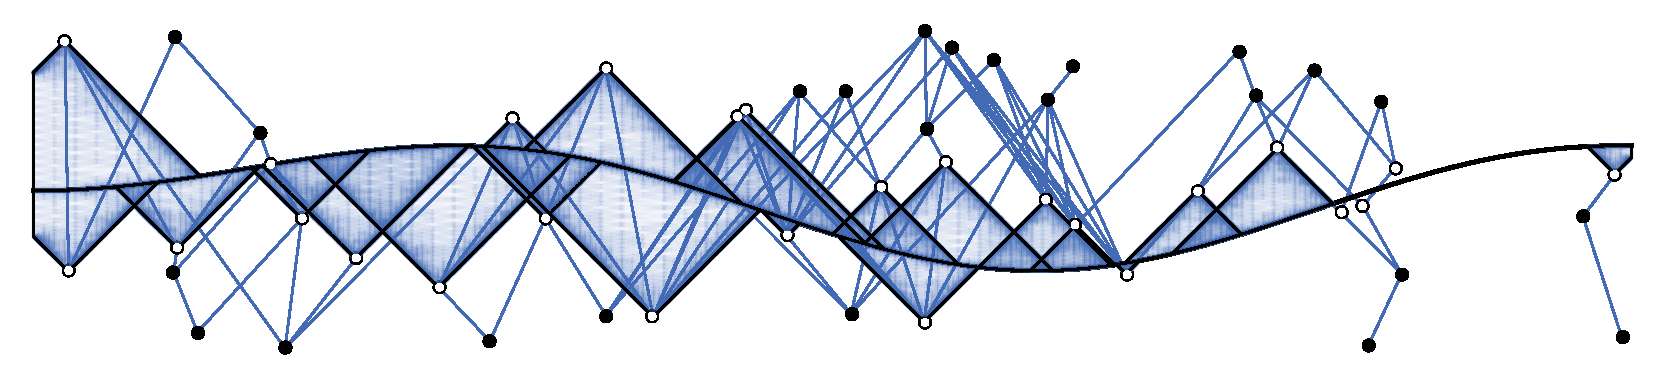
\includegraphics[width=\textwidth]{minmaxplot}}
    % \caption{An illustration of the idea. Pictured here is a causal set obtained by a sprinkling into a spacetime partitioned by a spacelike hypersurface. The minimal and maximal points about the surface are highlighted and the shaded regions illustrate the regions whose volumes $V_\blacktriangle$ and $V_\blacktriangledown$ are needed in the proof.}
     %\label{fig:Nmin_Nmax}
%*\end{figure}

\section{The Proof}

\subsection{Poisson Sprinklings for $\left\langle N_{max}^{\:(m)}\right\rangle$ and $\left\langle N_{min}^{\: (n)}\right\rangle$}

In order to prove~\eqref{eq:mainconjecture} and~\eqref{eq:conjecture_for_area} let us first derive expressions for the mean values of $N_{\vphantom{i}max}^{\: (m)}$ and $N_{min}^{(n)}$. The proof will will follow almost automatically, as~\eqref{general_boundary_sum} and~\eqref{general_area_sum} are just linear combination of $N_{\vphantom{i}max}^{\: (m)}$ and $N_{min}^{(n)}$ terms, and thus their mean values will just be linear combinations of $\left\langle N_{\vphantom{i}max}^{\: (m)}\right\rangle$ and $\left\langle N_{min}^{\: (n)}\right\rangle$ terms.

For any instance of the sprinkling, the probability that a sprinkled point $p\in M$ below the surface $\Sigma$ is $k$\emph{-next-to-maximal} is given by the probability that $k$ points of the sprinkling lie in the region $J^{+}(p)\cap J^{-}(\Sigma)$, the intersection of the causal future of $p$ with the causal past of the surface $\Sigma$.\footnote{For notational convenience we use the symbol $x$ to refer to the causal element $x\in\mathcal C$, to its embedding in the manifold $M$, and to its coordinates in some chart on $M$.} This region will in general be the interior of some curvy $d$-dimensional cone truncated by the surface $\Sigma$, as illustrated in Figure~\ref{fig:Nmin_Nmax}. We will refer to these regions as \emph{truncated cones}. The Poisson process assigns a probability
\be\label{Poisson}
\mathbb P\left(\text{k points in }J^{+}(p)\cap J^{-}(\Sigma)\right)=\frac{\left(\rho\: V_\blacktriangledown(p)\right)^k}{k!}e^{-\rho V_\blacktriangledown(p)}
\ee
to this event, where $V_\blacktriangledown(p)\equiv V(J^{+}(p)\cap J^{-}(\Sigma))$ is the spacetime volume of the region $J^{+}(p)\cap J^{-}(\Sigma)$. The probability of sprinkling an element into an infinitesimal four-volume $dV_p$ at $p$ is $\rho dV_p$ where $\rho=l^{-d}$ is the sprinkling density, and so the total expected number of $k$-next-to-maximal elements below $\Sigma$ is
\be\label{eq:nmax}
\langle N_{max}^{(k)}\rangle =\rho\int_{J^{-}(\Sigma)}dV_p\; \frac{\left(\rho\: V_\blacktriangledown(p)\right)^k}{k!}e^{-\rho V_\blacktriangledown(p)}
\ee
Similarly the expected number of $k$-next-to-minimal elements above $\Sigma$ is
\be\label{eq:nmin}
\langle N_{min}^{(k)}\rangle =\rho\int_{J^{+}(\Sigma)}dV_p\; \frac{\left(\rho\: V_\blacktriangle(p)\right)^k}{k!}e^{-\rho V_\blacktriangle(p)}
\ee
where $V_\blacktriangle(p)\equiv V(J^{+}(\Sigma)\cap J^{-}(p))$.

In the limit $\rho\rightarrow\infty$, both quantities will diverge, but if some combination of $k$-next-to-maximal/minimal terms grows slower than or at order $\rho^{1-\frac2d}$, the proposed action~\eqref{general_boundary_sum} will tend to a finite value in the continuum limit.

Consider a set of synchronous or Gaussian Normal Coordinates (GNC) $x^\mu=(t,\mathbf x)$ adapted to $\Sigma$ such that in a neighbourhood $U_\Sigma$ of $\Sigma$ the line element is
\be
ds^2 = -dt^2 + h_{ij}(t,\mathbf x) dx^i dx^j.
\ee
In these coordinates, the surface $\Sigma$ corresponds to $t=0$, and the coordinate $t$ measures the proper time elapsed along geodesics whose tangent vector is proportional to the surface normal on $\Sigma$.
%\be\label{GNC_metric}
%g_{\mu\nu}(x)=
%\begin{pmatrix}
 %-1&0 \\
% 0&h_{ij}(x)
%\end{pmatrix}.
%\ee
%In order to find $N_{max}$, the number of maximal points below the surface, one has to use the fact that the points have been sprinkled with a Poisson distribution. 
%If we pick a point $x_0=(0,\mathbf{x})\in \Sigma$ on the surface that has the same spatial coordinates as $x=(t,\mathbf{x})$ then the coordinate time, $t$, is the proper time elapsed along the unique geodesic between $x_0$ and $x$. The volume $V(\Sigma,x)$ then only depends on $t$.~\mb{error?}  
The integrals~\eqref{eq:nmax} and ~\eqref{eq:nmin} seem intractable as they stand, since the integration is over the entire causal past/future of the surface and the volume expressions will be complicated in the presence of curvature. However, for large $\rho$ (small $l$), the integrands $\exp(-\rho V)$ will be exponentially suppressed unless the volumes are small. Consider the spacetime region $U_\varepsilon=\left\{|t|<\varepsilon\right\}$ around the surface $\Sigma$ for some $\varepsilon>0$ (with $\varepsilon$ small enough such that the GNC system is valid throughout $U_\varepsilon$). We will assume that for any such $\varepsilon$, the contribution from points with $|t|>\varepsilon$ to the integrals~\eqref{eq:nmax} and \eqref{eq:nmin} can be made arbitrarily small by setting $\rho$ large enough, since the volumes of the truncated past/future lightcones for such points will be too large. Hence, as $\rho\rightarrow\infty$, the integration ranges in \eqref{eq:nmax} and \eqref{eq:nmin} can be cut off at finite time $t=\pm\varepsilon$ with $\varepsilon$ arbitrarily small, which allows us to expand the time integration-variable about zero. These assumptions of course impose certain regularity conditions on the surface $\Sigma$, but so long as $\Sigma$ is compact and everywhere spacelike  then these conditions are satisfied.\mb{do we need to say more about this? e.g. can't have asymp. null $\Sigma$ i guess} The integrals then simplify to
\begin{gather}\label{eq:nmax_and_eq:nmin}
\begin{aligned}
\langle N_{max}^{(k)}\rangle & =\rho \int_{\Sigma}d^{d-1}x\int_{-\varepsilon}^{0}dt\:
h^{\frac{1}{2}}\left(1+
\frac{1}{2}\frac{\dot{h}}{h}t+O(t^2)\right)
 \frac{\left(\rho\: V_\blacktriangledown(p)\right)^k}{k!} e^{-\rho V_\blacktriangledown(t,\mathbf x)}
\\
\langle N_{min}^{(k)}\rangle & =\rho \int_{\Sigma}d^{d-1}x\int_{0}^{\varepsilon}dt\:
h^{\frac{1}{2}}\left(1+
\frac{1}{2}\frac{\dot{h}}{h}t+O(t^2)\right) \frac{\left(\rho\: V_\blacktriangle(p)\right)^k}{k!} e^{-\rho V_\blacktriangle(t,\mathbf x)}
\end{aligned}
\end{gather}
where $h\equiv det\left(h_{ij}(0,\mathbf{x})\right)$ and $\dot{}\equiv \frac{\partial}{\partial t}$ and the metric determinant has been in expanded in small $t$.

The only truncated cones that contribute will have small volumes, as we are restricting ourselves close to the surface.
%\mb{this sounds circular w.r.t. last paragraph} 
This means that the volumes can be approximated in some scheme that will be made precise below. Any higher order corrections to these volumes, above the order we require, will vanish in the limit of $\rho\rightarrow\infty$.

\subsection{Lightcone Volumes}

In order to evaluate the volume $V_\blacktriangledown(p)$ or $V_\blacktriangle(p)$ of a truncated cone we will perform a coordinate transform to Riemann Normal Coordinates (RNCs) in a neighbourhood containing the cone. The discussion for the two volume integrals is identical so we will outline that for $V_\blacktriangle(p)$ (i.e. for points to the future of $\Sigma$). 

Fix $p\in M$ and denote its coordinate values in GNCs by $x^\mu_p=(t_p,\mathbf x_p)$. It will be convenient to use RNCs centered not at the tip $p$ of the cone but instead at the point $p_0$ where the unique geodesic through $p$ whose tangent is normal to $\Sigma$ intersects $\Sigma$. In GNCs this simply corresponds to the point $p_0$ with coordinates $x_0^\mu=x^\mu(p_0)=(0,\mathbf x_p)$. RNCs centered at $p_0$ will be given the symbol $y^{\overline{\mu}}$.
%\mb{let's put all facts about $x^\mu$ and $y^{\overline\mu}$ for $p$ and $p_0$ here and expansion of det in RNC.} 
We need to assume that for any $p$ in $U_\varepsilon$, the Riemann normal neighbourhood $U_p\subset M$ (throughout which the RNC system centered at $p_0$ is well-defined) contains the truncated cone $J^-(p)\cap J^+(\Sigma)$. This assumption seems reasonable given the that $U_\varepsilon$ can be made arbitrarily ``thin'' as $\rho\rightarrow\infty$. In RNCs the metric and the Christoffel symbols at $p_0$ are those of flat space:
\be\label{eq:RNCMetricTransAtPAndChris}
g_{\overline{\mu} \overline{\nu}}(p_0)=\eta_{\overline{\mu} \overline{\nu}}=A^{\mu}_{\;\overline{\mu}}A^{\nu}_{\;\overline{\nu}}g_{\mu\nu}(p_0)\;,\;\;\;\;\Gamma^{\overline{\mu}}_{\;\overline{\nu}\overline{\rho}}(p_0)=0
\ee
The $A^{\mu}_{\;\overline{\mu}}$ govern the coordinate transformation from GNCs to RNCs to linear order. %but $O(x^2)$ corrections may be required. 
To second order the coordinate transformation is given by
\be\label{eq:RNCtotaltrans}
y^{\overline{\mu}}=A^{\overline{\mu}}_{\;\nu}x^\nu+\frac{1}{2}A^{\overline{\mu}}_{\;\mu}\Gamma^{\mu}_{\;\nu\rho}(p_0)x^\nu x^\rho+O((x-x_0)^3).
\ee
The inverse relation to first order is 
\be\label{eq:RNCinversetrans}
x^{\mu}=A^{\mu}_{\;\overline{\nu}}y^{\overline{\nu}}+O(y^2)
\ee
and one finds that the $A^{\mu}_{\;\overline{\mu}}$ satisfy
\be\label{eq:RNCeqnforA}
A^{\overline{\mu}}_{\;\mu}A^{\mu}_{\;\overline{\nu}}=\delta^{\overline{\mu}}_{\;\overline{\nu}}\;,\;\;\;\;A^{\mu}_{\;\overline{\mu}}A^{\overline{\mu}}_{\;\nu}=\delta^{\mu}_{\;\nu}
\ee
These relations for RNC will cover all that will be needed in this discussion.

Now the volume of the truncated cone can be found as follows. 
%Consider the past lightcone emanating at the point $p_0=(T,\mathbf x_0)$ truncated by $\Sigma$. There is a unique point $q_0=(0,\mathbf x_0)$ on $\Sigma$ associated with $p_0$, separated from $p_0$ by proper time $T$. 
The volume of the cone is given by

\be\label{eq:VolumeWithNoSimplifications}
V_\blacktriangle(p)=\int_{\mathcal{X}_p} d^d x\;\sqrt{-g}
\ee
where the integration region, $\mathcal{X}_p\equiv  J^-(p)\cap J^+(\Sigma)$ will be a complicated expression. As we are dealing with points close to the surface we can use the  RNCs $y^{\overline{\mu}}$, defined as above, about the point $p_0$. Let us denote the time-coordinate of $p$ in GNCs by $T=x^0_p=t_p$. For the transformation from GNCs to RNCs at $p_0$ one finds that $A^{\overline 0}_{\;0}=1$, $A^{\overline 0}_{\;i}=0$ and $\delta_{\ibar\jbar}=A^i_{\;\ibar}A^j_{\;\jbar}h_{ij}(p_0)$, which in particular implies $y^{\overline{0}}_p=\overline{t}_p=t_p=T$. In RNC one can expand the metric determinant in~\eqref{eq:VolumeWithNoSimplifications} to find

\be\label{eq:VolumeWithRNC}
V_\blacktriangle(p) =\int_{\mathcal{X}_p}d^dy+\int_{\mathcal{X}_p}d^dy\left(-\frac{1}{6}R_{\overline{\mu}\overline{\nu}}(p_0)y^{\overline{\mu}}y^{\overline{\nu}} \right)+O(T^{d+3})
\ee
where $R_{\overline{\mu}\overline{\nu}}(p_0)$ is the Ricci tensor in RNC evaluated at $p_0$.\mb{justify beforehand which orders to keep?}
%The arguments of the volume function need not be changed as the volume only depends on the points in the manifold, $q_0$ and $p_0$. 
The second term comes in at $O(T^{d+2})$ so the volume we have to calculate has reduced to

\be\label{eq:VolumeToLowestOrder}
V_\blacktriangle(p) =\int_{\mathcal{X}_p}d^dy+O(T^{d+2})
\ee
Terms of $O(T^{d+2})$ can be retained till the end, but in the limit, $\rho\rightarrow\infty$, they vanish. This will be proved below.

This is now a simple volume integral but we need to find the boundaries of $\mathcal{X}_p$ to write down the integration limits. There are two parts to the boundary of the (solid) truncated cone: the lightcone emanating at $p$ and the base, given by the intersection of $\Sigma$ with the interior of the lightcone. First we look at the lightcone. Following \cite{Khetrapal_Sumati:Causal_Diamond_Volume} it can be shown that the first curvature correction to the lightcone comes in at $O(T^{d+2})$ and so can be ignored for our purposes. This means that the lightcone can be treated as effectively flat in RNCs and thus corresponding to the set $(y^{\overline{1}})^2+(y^{\overline{2}})^2+...+(y^{\overline{d-1}})^2= T-\overline{t}$.\mb{what limit on $\bar t$?}

The base of the cone in GNCs is simply a part of the surface $t=0$, so we can use (\ref{eq:RNCtotaltrans}) to find the equation for the surface in RNCs. Equation (\ref{eq:RNCtotaltrans}) gives

\be\label{eq:BottomSurfaceWithGNC}
\overline{t}=\frac{1}{2}\Gamma^{0}_{\;ij}(p_0)x^i x^j+O( x^3)\ee

The linear part on the right of (\ref{eq:RNCtotaltrans}) vanishes as $A^{\overline{0}}_{\;\mu}x^{\mu}=x^0$ (as $A^{\overline{0}}_{\;i}=0$ and $A^{\overline{0}}_{\;0}=1$) and $x^0=t=0$ for the bottom surface. Using the inverse RNC relation (\ref{eq:RNCinversetrans}) one can find the equation for the bottom surface in RNCs:

\be\label{eq:BottomSurface}
\overline{t}=\frac{1}{2}\Gamma^{0}_{\;ij}(p_0)A^{i}_{\;\ibar}A^{j}_{\;\jbar}y^{\ibar} y^{\jbar}+O(y^3)
\ee

Let us rewrite this equation in spherically symmetric coordinates, i.e. define $r=\sqrt{\delta_{\ibar\jbar}y^\ibar y^\jbar}$ and the usual angular coordinates $\phi_1,..,\phi_{d-2}$ in terms of the spatial coordinates $y^{\overline{1}} = r \cos(\phi_1),\ldots, y^{\overline{d-1}} = r \sin(\phi_1) \cdots \sin(\phi_{d-3}) \sin(\phi_{d-2})$. Then

\be\label{eq:RadialBottomSurface}
\overline{t}=\frac{1}{2}\left(\Gamma^{0}_{\;ij}(p_0)A^{i}_{\;\ibar}A^{j}_{\;\jbar}\frac{y^{\ibar} y^{\jbar}}{r^2}\right)r^2+O(y^3)=\frac{1}{2}f(\mathbf{x}_p,{\boldsymbol\phi})r^2+O(y^3)
\ee
where $\boldsymbol\phi$ stands collectively for all the angular coordinates $\phi_1,..,\phi_{d-2}$. The function $f(\mathbf{x}_p,\boldsymbol\phi)$ depends on $\mathbf{x}_p$ since $\Gamma^{0}_{\;ij}$ and $A^{i}_{\;\ibar}$ depend on $p_0$.
%One can see that $f(\mathbf{x}_0,\boldsymbol\phi)$ depends on the angles, $\phi$, by substituting the relations below into (\ref{eq:RadialBottomSurface})
%\begin{equation}
%\begin{aligned}\label{eq:SphericalCoords}
%y^{\overline{1}} &= r \cos(\phi_1)  \\
%y^{\overline{2}} &= r \sin(\phi_1) \cos(\phi_2)  \\
%y^{\overline{2}} &= r \sin(\phi_1) \sin(\phi_2) \cos(\phi_3)  \\
%    &\vdots  \\
%y^{\overline{d-2}} &= r \sin(\phi_1) \cdots \sin(\phi_{d-3}) \cos(\phi_{d-2})  \\
%y^{\overline{d-1}} &= r \sin(\phi_1) \cdots \sin(\phi_{d-3}) \sin(\phi_{d-2})
%\end{aligned}
%\end{equation}

With the boundaries of the integration region in place, we can now write down the integral explicitly in spherical coordinates:

\be\label{eq:VolumeIntegralSpherical}
V_\blacktriangle(p)=\int_{S^{d-2}}
d\Omega_{d-2}
\int_{0}^{r_{max}(\phi)}r^{d-2}dr
\int_{\frac{1}{2}f(\mathbf{x}_p,\phi)r^2}^{-r+T}
d\overline{t}+O(T^{d+2})
\ee
where $r_{max}(\boldsymbol\phi)$ is the value of the radial coordinate for which the surface $\Sigma$ intersects the lightcone at angle $\boldsymbol\phi$, as shown in Figure \ref{fig:cone_plot}. To find this value one needs to solve 
\be
\frac{1}{2}f(\mathbf{x}_p,\boldsymbol\phi){r_{max}}^2(\boldsymbol\phi)=-r_{max}(\boldsymbol\phi)+T
\ee 
for $r_{max}(\boldsymbol\phi)$ and take the positive solution. The solution can be expanded in $T$ and is simply $r_{max}=T+O(T^2)$, with angular dependent terms contributing at $O(T^2)$. The $O(T^2)$ term will contribute at $O(T^{d+2})$ in the volume integral and so can be ignored. Substituting $r_{max}=T$ into (\ref{eq:VolumeIntegralSpherical}) allows us to evaluate the integral, wherein we find 
%\begin{figure}[t]
 % \centering
  %  {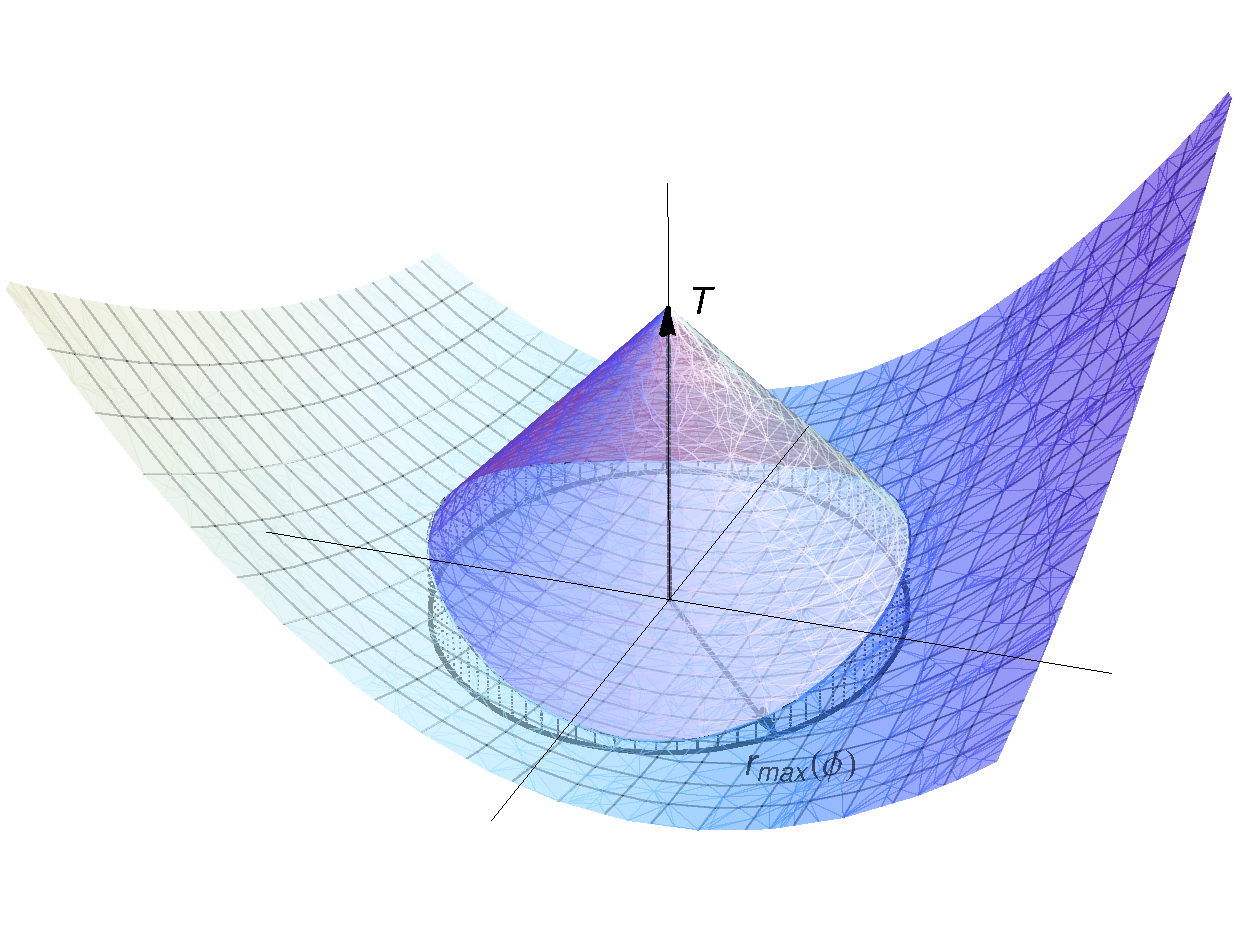
\includegraphics[scale=0.5]{coneplot}}
   %  \caption{The size of the region inside the top and bottom bounding surfaces is the volume we want to calculate.}
    % \label{fig:cone_plot}
%\end{figure}
\be\label{eq:VolumeNoK}
V_\blacktriangle(p)
=\frac{V_{d-1}}{d}T^d\left(1-\frac{d}{2(d+1)}\Gamma^{0}_{\;ij}(p_0)A^{i}_{\;\ibar}A^{j}_{\;\jbar}\delta^{\ibar\jbar}T\right)
+O(T^{d+2})
\ee
where the $\delta^{\ibar\jbar}$ comes from the fact that cross terms ($\ibar\neq \jbar$) vanish under the angular integration. The defining relations for $A^{i}_{\;\ibar}$ can now be rearranged to give $A^{i}_{\;\ibar}A^{j}_{\;\jbar}\delta^{\ibar\jbar}=h^{ij}(p_0)$. In GNCs the extrinsic curvature on the surface is given by

\be\label{eq:K}
K
=g^{\mu\nu }\nabla_{\mu}n_{\nu}
=-\Gamma^{0}_{\;ij}h^{ij}=-\frac{1}{2}\frac{\dot{h}}{h}.
\ee
Substituting this into~\eqref{eq:VolumeNoK} we obtain 
\begin{align}
V_\blacktriangle(T,\mathbf x)
&=\frac{V_{d-1}}{d}T^d\left(1+\frac{d}{2(d+1)}K(0,\mathbf{x})T\right)
+O(T^{d+2}) \label{eq:TopVolumeWithK}\\
V_\blacktriangledown(-T,\mathbf x)
&=\frac{V_{d-1}}{d}T^d\left(1-\frac{d}{2(d+1)}K(0,\mathbf{x})T\right)
+O(T^{d+2}), \label{eq:BottomVolumeWithK}
\end{align}
having dropped the subscript $p$. Given the volume expressions in GNCs we now proceed to evaluate the integrals for $\langle N_{min}^{(k)}\rangle $ and $\langle N_{\vphantom{i}max}^{(k)}\rangle$.

\subsection{The mean of $S^{(d)}_{GHY}[\mathcal {C}^-,\mathbf{p};\mathcal{C}^+,\mathbf{q}]$}

Using the previous equations for the volumes of the truncated cones we find that~\eqref{eq:nmax_and_eq:nmin} reduces to

\begin{gather}\label{eq:nmax_and_eq:nmin_volume_expanded}
\begin{aligned}
\langle N_{max}^{(k)}\rangle = \frac{\rho^{k+1}}{k!} & \int_{\Sigma}d^{d-1}x\int_{-\varepsilon}^{0}dt\:
h^{\frac{1}{2}}\left(1+
\frac{1}{2}\frac{\dot{h}}{h}t\right)
 \\
 & \times \Big( A(-t)^d \Big)^k 
 \Big( 1 - B(-t) \Big)^k
 e^{-\rho A(-t)^d \left[1-B(-t) \right]} + .\,.\,.
\\
\langle N_{min}^{(k)}\rangle = \frac{\rho^{k+1}}{k!} & \int_{\Sigma}d^{d-1}x\int_{0}^{\varepsilon}dt\:
h^{\frac{1}{2}}\left(1+
\frac{1}{2}\frac{\dot{h}}{h}t\right)
 \\
 & \times \Big( A\: t^d \Big)^k 
 \Big( 1 + B\: t \Big)^k
 e^{-\rho A\: t^d \left[1+B\: t \right]} + .\,.\,.
\end{aligned}
\end{gather}
where we have defined
\begin{gather}\label{A_and_B_defn}
\begin{aligned}
A & := \frac{V_{d-1}}{d} \\
B & := \frac{V_{d-1}}{2(d+1)}K(0,\mathbf{x})
\end{aligned}
\end{gather}
Once again the higher order terms that have been ignored in both equations will be shown to vanish in the limit. From~\eqref{eq:K} we can substitute $K$ in for $\frac{1}{2}\frac{\dot{h}}{h}t$. We swap the integration variable to $t\rightarrow -t$ in the first equation and expand the $O(t^{d+1})$ part of the exponentials to give

\begin{gather}\label{eq:nmax_and_eq:nmin_volume_expo_expanded}
\begin{aligned}
\langle N_{max}^{(k)}\rangle = \frac{\rho^{k+1}}{k!} & \int_{\Sigma}d^{d-1}x\int_{0}^{\varepsilon}dt\:
h^{\frac{1}{2}}\left(1+
K\: t\right)
 \\
 & \times \Big( A\: t^d \Big)^k 
 \Big( 1 - B\: t \Big)^k
 \Big( 1 + \rho A B\: t^{d+1} \Big)
 e^{-\rho A\: t^d} + .\,.\,.
\\
\langle N_{min}^{(k)}\rangle = \frac{\rho^{k+1}}{k!} & \int_{\Sigma}d^{d-1}x\int_{0}^{\varepsilon}dt\:
h^{\frac{1}{2}}\left(1-
Kt\right)
 \\
 & \times \Big( A\: t^d \Big)^k 
 \Big( 1 + B\: t \Big)^k
  \Big( 1 - \rho A B\: t^{d+1} \Big)
 e^{-\rho A\: t^d} + .\,.\,.
\end{aligned}
\end{gather}
The reason for expanding the exponentials is that the integrals will have to be put into the form of Gaussian integrals in order to evaluate them in the limit $\rho\rightarrow\infty$. The above expressions are almost the same apart from a few sign differences, so from now on we will just work with the expression for $\langle N_{min}^{(k)}\rangle$. By expanding the brackets, and retaining only necessary orders, the integral can be split into two parts of differing powers of $\rho$.

\begin{gather}\label{eq:n_min_different_rho_terms}
\begin{aligned}
\langle N_{min}^{(k)}\rangle & = \frac{\rho^{k+1}A^k}{k!}\int_{\Sigma}d^{d-1}x\: h^{\frac{1}{2}}\int_{0}^{\varepsilon}dt\:
\left\lbrace \left( t^{dk} + \left(kB-K \right)t^{dk+1}\right) + O\left(t^{dk+2}\right) \right\rbrace e^{-\rho A\: t^d}
 \\
 & - \frac{\rho^{k+2}A^{k+1}}{k!}\int_{\Sigma}d^{d-1}x\: h^{\frac{1}{2}}\int_{0}^{\varepsilon}dt\:
\left\lbrace Bt^{dk+d+1} + O\left(t^{dk+d+2}\right) \right\rbrace e^{-\rho A\: t^d}
\end{aligned}
\end{gather}
To find out how this diverges in the limit of $\rho \rightarrow\infty$, it suffices to find the divergence of the following general expression
\be\label{eq:general_t_n_integral}
\lim_{\rho\rightarrow\infty}\rho^{p}\int_{0}^{\varepsilon}dt\
t^{q}e^{-\rho At^{d}}
\ee
where $p,q \in \mathbb{R}$. We make the substitution $z=\rho At^{d}$ to put~\eqref{eq:general_t_n_integral} into the form of an incomplete gamma function.

\be\label{eq:incomplete_gamma_function}
\lim_{\rho\rightarrow\infty}\frac{A^{-\left(\frac{q+1}{d} \right)}}{d}\rho^{p-\left(\frac{q+1}{d} \right)}\int_{0}^{\rho A \varepsilon^d}dz\
z^{\left(\frac{q+1}{d} \right)-1}e^{-z}
\ee
The pre-factor has come from the substitution. In the limit we can retain the $\rho$ outside the integral while taking the integration limit to $\infty$. In doing this the integral becomes a gamma function.

\be\label{eq:gamma_function}
\lim_{\rho\rightarrow\infty}\frac{A^{-\left(\frac{q+1}{d} \right)}}{d}\rho^{p-\left(\frac{q+1}{d} \right)}\int_{0}^{\infty}dz\
z^{\left(\frac{q+1}{d} \right)-1}e^{-z}=\lim_{\rho\rightarrow\infty}
\frac{A^{-\left(\frac{q+1}{d} \right)}}{d}\rho^{p-\left(\frac{q+1}{d} \right)}\Gamma\left( \frac{q+1}{d} \right)
\ee
We can use this procedure to take the limit of~\eqref{eq:n_min_different_rho_terms} and formulate the answer in terms of gamma functions. The limits of both $\langle N_{\vphantom{i}max}^{(k)}\rangle$ and $\langle N_{min}^{(k)}\rangle$ are then given by

\begin{gather}\label{eq:nmax_nmin_final}
\begin{aligned}
\lim_{\rho\rightarrow\infty}\langle N_{max}^{(k)}\rangle = \lim_{\rho\rightarrow\infty} & \left\lbrace \rho^{1-\frac{1}{d}} \left(b_d\right)^{-1} \frac{\Gamma\left(\frac{1}{d}+k\right)}{k!}
\int_{\Sigma}d^{d-1}x\: \sqrt{h} \right.
 \\
 &  \left. +\rho^{1-\frac{2}{d}} \left(c_d\right)^{-1} \frac{\Gamma\left(\frac{2}{d}+k\right)}{k!}
\int_{\Sigma}d^{d-1}x\: \sqrt{h}K + O\left(\rho^{1-\frac{3}{d}} \right) \right\rbrace
\\
\lim_{\rho\rightarrow\infty}\langle N_{min}^{(k)}\rangle = \lim_{\rho\rightarrow\infty} & \left\lbrace \rho^{1-\frac{1}{d}} \left(b_d\right)^{-1} \frac{\Gamma\left(\frac{1}{d}+k\right)}{k!}
\int_{\Sigma}d^{d-1}x\: \sqrt{h} \right.
 \\
 &  \left. -\rho^{1-\frac{2}{d}} \left(c_d\right)^{-1} \frac{\Gamma\left(\frac{2}{d}+k\right)}{k!}
\int_{\Sigma}d^{d-1}x\: \sqrt{h}K + O\left(\rho^{1-\frac{3}{d}} \right) \right\rbrace
\\
\end{aligned}
\end{gather}

These objects diverge as $\rho^{1-\frac{1}{d}}$ in the limit. The factor of $\rho$ that must be included in the formula for the surface volume is exactly the inverse of this ($\rho^{\frac{1}{d}-1}$), as can be seen from~\eqref{general_area_sum} if one substitutes in $l=\rho^{-\frac{1}{d}}$. If we include this factor above, and take the limit, we see that the only remaining terms are proportional to the surface volume. The other terms all have negative powers of $\rho$ and therefore vanish as $\rho\rightarrow\infty$. This means that if we take the mean of~\eqref{general_area_sum}, in the limit of $\rho\rightarrow\infty$, and substitute in the above expressions, we will be left with something proportional to the surface volume. Then it is easy to see that in order to get the surface volume exactly one must force $\mathbf{p}$ and $\mathbf{q}$ to satisfy~\eqref{area_coefficient_relation}. This concludes the proof of the spatial volume claim,~\eqref{eq:conjecture_for_area}. 

If we take the mean of~\eqref{general_boundary_sum} and the limit $\rho\rightarrow\infty$, we can substitute in the above expressions to find that the only terms left that have non-negative powers of $\rho$ (and therefore non-vanishing in the limit) are that of the spatial volume and boundary term. The term proportional to the spatial volume is divergent, so the coefficients, $\mathbf{p}$ and $\mathbf{q}$, must satisfy~\eqref{coefficient_relation1} to make this term vanish. The other condition,~\eqref{coefficient_relation2}, ensures that what remains is equal to the GHY boundary term. Thus, the proof of~\eqref{eq:mainconjecture} is complete.

The form of~\eqref{eq:nmax_nmin_final} seems to suggest general series expansions of $\langle N_{max}^{(k)}\rangle$ and $\langle N_{min}^{(k)}\rangle$ in reducing powers of $\rho$. Written in terms of the discreteness scale, $l$, it is a Laurent series starting at $l^{1-d}$. The higher order terms, in $l$, will possibly be proportional to higher order normal derivatives of the surface volume. If this were true then one could find discrete versions for normal derivatives of the surface volume to any order. The exact form of the constant in the next term of the series is unknown and more work must be done to determine a general trend for the constants, and hence find the general series.

\section{Fluctuations}
So far we have only talked about the mean of the causal set boundary action for sprinklings. Let us now turn to its fluctuations (the standard deviation) $\sigma[\mathbf S^{(d)}_{GHY}]=\text{Var}[\mathbf S^{(d)}_{GHY}]^\frac12$.\footnote{Whenever we say fluctuations we refer to the standard deviation of the random variable, not to its variance.} If we restrict ourselves for now to the particular boundary action $\mathbf S^{(d)}_{0}$, which is proportional to the difference between the random variables $\mathbf N^{(0)}_{\vphantom{i}max}$ and $\mathbf N_{min}^{(0)}$ associated with $M^-$ and $M^+$, we can give a heuristic argument to estimate the dependence of fluctuations on $\rho=l^{-d}$. In any spacetime region of fixed volume $V$ the number of causal set elements $N$ experiences Poisson fluctuations of order $\sqrt N$. Since $\mathbf N_{max}^{(0)}$ and $\mathbf N_{min}^{(0)}$ are quantities associated with a codimension-1 surface (they count elements ``near" $\Sigma$), we may expect them to scale like $N^\frac{d-1}{d}$ (which indeed agrees with the leading order behaviour of~\eqref{eq:nmax_nmin_final}) and thus to inherit fluctuations of order $N^\frac{d-1}{2d}$. 
%{This comes from the following observation. In a volume corresponding to a thickening of the hypersurface $\Sigma$ by one unit of the discreteness scale $l$ (e.g. by Lie dragging the surface along its normal by an amount $l$),.... }
The action $\mathbf S^{(d)}_{0}$, being proportional to $\rho^\frac{2-d}{d}$ times the difference of two \emph{independent}\footnote{The independence is as a feature of the Poisson process in $M$: the number of elements $N(R)$ in any subregion $R\subset M$ is a Poisson variable itself, and for any two disjoint regions $R_1$, $R_2$ the numbers $N(R_1)$ and $N(R_2)$ are independent random variables.} random variables with standard deviation $N^\frac{d-1}{2d} = (\rho V)^\frac{d-1}{2d}$ should then see fluctuations of order $\rho^\frac{2-d}{d}\rho^\frac{d-1}{2d}=\rho^\frac{3-d}{2d}$. This suggests that for $d=2$ these fluctuations should grow like $\rho^{\frac{1}{4}}$ as $\rho\rightarrow\infty$, for $d=3$ they should be constant, and for $d>3$ they should be damped.

In order to test this heuristic argument one may like to write down the integral expression for $\text{Var}[\mathbf S^{(d)}_{GHY}]$, but it is complicated enough even for $\mathbf S^{(d)}_0$ in finite regions of flat space that it will not be very illuminating to reproduce here. It also seems far less tractable than the expression for the mean because it involves terms of the type $\int d^dx\int d^dy \exp\left[-\rho V(J^+(x)\cap J^+(y))\right]$ for which the above methods of cutting off the time-integration range and Taylor expanding will not follow through. Instead we will show the results of computer simulations that support results of the heuristic argument. 

%\begin{figure}[t!]
 % \centering
  %  {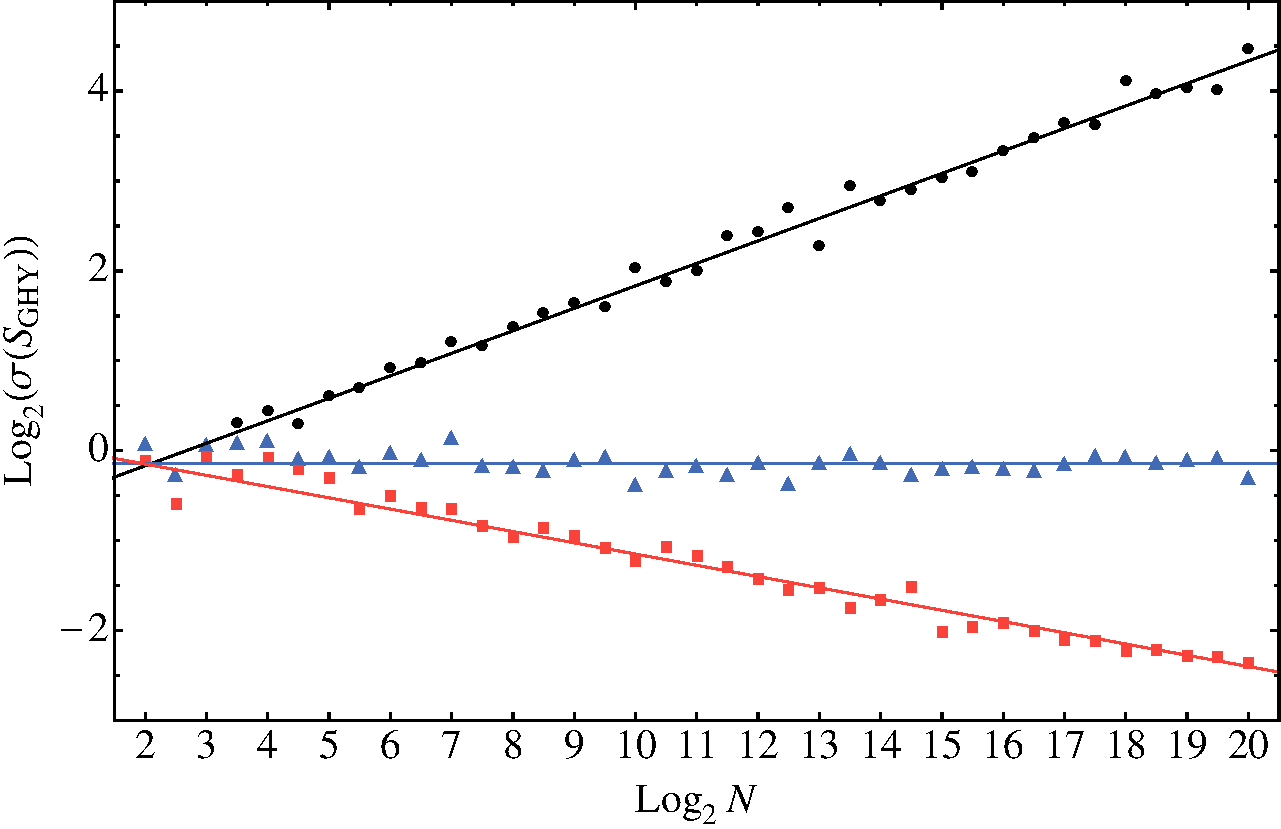
\includegraphics[scale=0.6]{GHY-fluctuation_plots}}
   %  \caption{A $\log-\log$ plot (base $2$) of the fluctuations in $S^{(d)}_{GHY}$ for a flat ($K=0$) surface in $d=2,3$ and $4$-dimensional Minkowski space. Each data point represents the sample standard deviation in $S^{(d)}_{GHY}$ on a sample of $R=100$ runs. Black dots, blue triangles and red squares correspond to the simulation results in $d=2,3$ and $4$ dimensions, respectively. The corresponding black, blue and red lines have gradients $\frac12$, $0$ and $-\frac18$ and best-fit intercepts of order $1$.}
    % \label{fig:fluctuations}
%\end{figure}

 
The simulations were carried out as follows. Denote the discreteness scale by $l$. Take a $d$-cube $[0,L]^d$ in $d$-dimensional Minkowski space with metric $ds^2=-dt^2+d{\mathbf x}^2$ and define the hypersurface $\Sigma: t=L/2$, which partitions the cube into two equal halves. Sprinkle at density $\rho=l^{-d}$ into the cube, which will place $\mathbf N$ points inside the cube, where $\mathbf N$ is a Poisson random number with mean $\left< \mathbf N\right> = \rho V=  (L/l)^d$. We evaluate the random variable $\mathbf S^{(d)}_{0}=\rho^\frac{2-d}{d}c_d\left(2\Gamma\left(\frac{2}{d}\right)\right)^{-1}(\mathbf N^{(0)}_{\vphantom{i}max} - \mathbf N_{min}^{(0)})$ by counting the minimal/maximal elements in the upper/lower half of the cube, and repeat for $R$ runs. The expected value for the mean is zero in all cases, since the extrinsic curvature of the surface is zero. 

In Figure~\ref{fig:fluctuations} we display the simulation results for $d=2,3,4$ spacetime dimensions, with $N=\rho$ ranging up to $2^{20}\approx 1$ million, having set $V=L^d=1$. Each data point represents the fluctuations (the standard deviation) in a sample of $R=100$ runs. The solid lines have been obtained by fitting an arbitrary constant multiplier in the scaling law predicted by the argument above, $\gamma(d)\times N^\frac{3-d}{2d}$, to the data sets. The best fit values are all of order $1$: $\gamma(2)=0.63$, $\gamma(3)=0.91$, and $\gamma(4)=1.07$.
There is clearly a good fit between the data and the scaling predicted by the heuristic argument. Although not visible on the plot, the data points were all consistent with zero mean as well.

For completeness we have performed analogous simulations for $\mathbf S^{(d)}_-$, which involves counting $\mathbf N^{(1)}_{max}$ and $\mathbf N^{(0)}_{max}$. In this case, heuristic arguments of the type given above are hampered by the fact that the two random variables whose difference is taken are not independent. However, the results for the scaling of the fluctuations turn out to be identical to those obtained for $\mathbf S^{(d)}_0$. 

\section{Timelike Boundaries}





\section{A Candidate Boundary Term for an Alexandrov Interval}
\newcommand{\vol}{\mathrm{vol}}

Until now our approach has been to reconstruct the  continuum GHY term  from the information in a causal set. 
The candidate described in the previous sections for a spatial boundary has a natural expression in a causal set  in  terms of its maximal and minimal elements which are the  analogs of a  space-like boundary.  A suitable analog  of  a time-like boundary  term has been harder to  construct; there is no simple causal set  characterisation of such  a boundary. Indeed, it is difficult to give a causal set  characterisation of a  spacetime region bounded by time-like surfaces. On the other hand, this is not true of causally defined spacetime regions since  past and future sets are defined naturally in  a causal set. An important example of such a region is the  Alexandrov interval which is used extensively  in calculations of causal set kinematics.  In the continuum such a region  is bounded by null hypersurfaces and their codimension 2 joints.  

Conversely in the continuum,   while the GHY term  is well defined for both a space-like and time-like boundary  (including their co-dimension 2 joints)  it is an open question what the contribution from a null  boundary  is \cite{Gibbons_Hawking_Boundary, Harris}. Apart from some sketchy suggestions in the literature \cite{neiman} there is no rigourous construction of such a term; indeed the standard variational route for finding the boundary contribution to the action appears to fail for null boundaries. 

Given our ignorance in this matter,  we can ask if causal set theory  might  in fact guide us in the right direction.   Our starting point is the $d$-dimensional  Benincasa-Dowker Action \cite{Benincasa_Dowker:The_Scalar_Curvature_of_a_Causal_Set, Dowker_Glaser:dAlembertians_for_Causal_Sets} which is constructed from the mean number  $N_i^{(d)}${\footnote{ $N_i^{(d)}$ is dimension  and geometry dependent, but for our purpose it suffices to retain the dimension label. } of $i+1$-element inclusive intervals in the causal set 
\begin{equation}   
8 \pi G {S_{BD}^{(d)}}[\mathcal C] = -\alpha_d \rho^{\frac{2-d}{d}}\biggl( N[\mathcal C]+ \frac{\beta_d}{ \alpha_d} \sum_{i=1}^{n_d-1}  C^{(d)}_{i} N _i^{(d)}[\mathcal C] \biggr) 
\label{bd} 
\end{equation}  
with   
\begin{equation}
\begin{aligned}
 \alpha_d =   
\begin{cases}
-\frac{1}{\Gamma(\frac{2+d}{d})}c_d ^{2/d}  \quad   &d \, \, \mathrm{odd} \\
-2 \frac{1}{\Gamma(\frac{2+d}{d})}c_d ^{2/d}  \quad   &d \, \,  \mathrm{even} \\
\end{cases}
\qquad\text{and}\qquad \beta_d = 
\begin{cases} 
\frac{d+1}{2^{d-1}\Gamma(2/d +1)} c_d^{2/d}   \quad   &d\mathrm{ \, \, odd}\\ 
\frac{\Gamma(d/2+2)\Gamma(d/2+1)}{\Gamma(2/d)\Gamma(d)}c_d^{2/d}  &  d\mathrm{ \, \,  even}\\ 
\end{cases} 
\end{aligned}
\end{equation}
and
\begin{equation} 
n_d = 
\begin{cases} 
\frac{d-1}{2} + 2  \quad & d\mathrm{ \, \, odd}\\ 
\frac{d}{2} + 2  \quad &d\mathrm{ \, \,  even,}\\ 
\end{cases} 
\end{equation} 
where  $2^{-d/2} c_d$ is the volume of a unit Alexandrov interval $I(x,y)$, i.e., one for which the proper time $\tau(x,y)=1$. 
%%{ {\bf \color{red} this is not correct! $c_d= \vol(S^{d-2}) \frac{ 2^{\frac{2-d}{2}}}{d(d-1)}$ and $\vol(S^{d-2})$ the volume of the homogeneous $d-2$ sphere}}.  
The coefficients $C_i^{(d)}$ of the terms $N_i^{(d)}$ in the sum are
\begin{equation}
\label{cid}
 C_i^{(d)}= 
\begin{cases} 
\sum_{k=0}^{i-1} (-1)^k\binom{i-1}{k} \frac{\Gamma(d/2(k+1)+3/2)}{\Gamma(d/2+3/2) \Gamma(1+dk/2)}  \quad  &\mathrm{d \, \, odd}\\ 
\sum_{k=0}^{i-1} (-1)^k\binom{i-1}{k} \frac{\Gamma(d/2(k+1)+2)}{\Gamma(d/2+2) \Gamma(1+dk/2)}  & \mathrm{d \, \,  even.}\\ 
\end{cases} 
\end{equation} 
These coefficients can be expressed more compactly as hypergeometric functions 
\begin{equation}
C_i^d={}_{q+1}F_{q}(\{ a_1, \ldots a_q, i-1\}, \{b_1, \ldots b_q \} |1)
\label{chyp} 
\end{equation} 
with $q=d/2+1/2, a_i=\frac{d+2i}{d}, b_i=2i/d$ for $d$ odd and $q=d/2, a_i=\frac{d+2i+2}{d}, b_i=2i/d$  for $d$ even.  


If $S_{BD}^{(d)}$ were precisely the discrete analog of the Einstein Hilbert action {\it without} any boundary contributions, then in flat spacetime  $S_{BD}^{(d)}$ should  vanish. However, as shown explicitly in \cite{bbdtwo} this is not the case for Alexandrov intervals in $d=2$  flat spacetime. Indeed, there is a residual contribution that goes to a non-vanishing constant in the continuum limit $N\rightarrow \infty$.  When the action is evaluated in rectangular regions in the same spacetime or for Alexandrov intervals in  the flat trousers spacetime, this is no longer the case. Thus, it seems plausible that the $d=2$ BD action contains boundary information. Moreover, in the case of Alexandrov intervals the asymptotic value of the action is the same  irrespective of the interval size. While this might suggest a  topological origin, we will now show that it is a part of a more general  result for $d>2$ and  has a geometrical origin. Namely it corresponds to the volume  $\vol(S^{d-2})$ of the $S^{d-2}$ joint which is independent of the interval size {\it only} in $d=2$.   

Consider an Alexandrov interval $I(p,q)=I^+(p) \cap I^-(q)$ for two events $p,q$ in a causal spacetime.   While the  boundary of $I(p,q)$ may be quite complicated in general, some of these components must necessarily be null.  In flat spacetime, for example,  the boundary of $I(p,q)$ consists of the two events $p$ and $q$, the subsets $B^\pm$ of the  two null hypersurfaces $\partial J^+(p)$ and $\partial J^-(q)$, and their intersection or ``joint''  $S^{d-2}=\partial J^+(p) \cap \partial J^-(q)$ which is a codimension 2 sphere.  Evaluating the BD action in an Alexandrov interval in flat spacetime should therefore yield  only boundary dependent terms.  In flat spacetime the $S^{d-2}$ joint  has radius $\tau(p,q)/2$, and thus increases with the size of the Alexandrov interval ${\mathrm{vol}}(I(p,q)) = N/\rho$, where $N$ is the mean of the number of causal set elements sprinkled into $I(p,q)$ . In what follows we take the continuum limit $\rho, N \rightarrow \infty$ while keeping ${\mathrm{vol}}(I(p,q))$ fixed. \ss{It would be nice to have a fancy picture of an Alex. interval here..}  
%% If $p$ or $q$ were to be taken to time-like past or future infinity, this volume would go to infinity as expected.

In \cite{Glaser_Sumati:Locality_in_Causal_Set} a closed form expression was obtained for the mean value of the number of $i+1$ element inclusive intervals $N_i^d$ contained in an Alexandrov interval in $d$ dimensional flat spacetime 
\begin{equation} N_i^d= \frac{\Gamma(d)^2\, \, N^{i+2}}{\Gamma(i)} \sum_{k=0}^\infty \frac{(-N)^k \, \, \, \Gamma(\frac{d(k+i)}{2}+1) \, \, \,  \Gamma(\frac{d(k+i+1)}{2}+1)}{(k+i+2) \, (k+i+1)\, \Gamma(k+1)\, \Gamma(\frac{d(k+i)}{2} +d) \,\Gamma(\frac{d(k+i+1)}{2}+d)}, 
\end{equation} 
where $i \geq 1$.  We use this to expand the sum in (\ref{bd}) as a power series in $N$: $\sum_{i=1}^{n_d} C_i^d \, \, N_i^{(d)} = \sum_{j=1}^\infty A_j^d \, \, N^{j+1}$.  After a rearrangement and redefinition of indices we find that 
\begin{equation}
 A_j^d = \Gamma(d)^2\biggl( \sum_{i=1}^{D+2} (-1)^i \binom{j-1}{i-1}  C_i^d  \biggr) \frac{(-1)^j}{(j+1)!}\frac{\Gamma(\frac{d}{2}(j-1)+1)\Gamma(\frac{d}{2}j+1)}{\Gamma(\frac{d}{2}(j-1)+d) \Gamma(\frac{d}{2}j+d)}, 
\end{equation} 
where $d=2D$ for $d$ even and $d=2D+1$ for $d$ odd.   
% Using the abbreviated form $C_i^d=\sum_{l=0}^{i-1} \binom{i-1}{l}A(d,l)$ where $A(d,l)$ is defined using \ref{cid} 
% we find that 
% \begin{equation}
% \sum_{i=1}^{D+2} (-1)^i \binom{j-1}{i-1}  C_i^d = (-1)^{j-1} A(d,j-1),  
% \end{equation}      
% where we have used the binomial identities  BLAH. Thus 
% \begin{equation}
%  \sum_{i=1}^{n_d} C_i^d N_i^{(d)}= ((d-1)!)^2 \sum_{j=1}^\infty(-1)^j B(d,j) \frac{\Gamma(\frac{d}{2}j+1)}{\Gamma(j+2)\Gamma(\frac{d}{2}(j-1)+d)\Gamma(\frac{d}{2}j+d)}N^{j+1}
% \label{thesum} 
% \end{equation} 
% where 
% \begin{equation} 
% B(d,j) = \left \{ 
% \begin{array}{ccc} 
% \frac{\Gamma(\frac{d}{2}j+3/2)}{\Gamma(\frac{d}{2}+3/2)}  &\quad & d \, \, odd, \\  \frac{\Gamma(\frac{d}{2}j+2)}{\Gamma(\frac{d}{2}+2)}  &\quad & d \, \, even.  \\ 
% \end{array} 
% \right
% \end{equation} 
This can be simplified to 
\begin{equation}
A_j^d= \gamma_j^d \, \, \Gamma(d)^2 (-1)^{j+1} \frac{1}{\Gamma(\frac{d}{2} (j + 1)) \Gamma(\frac{d}{2} (2 + j)) \Gamma(2 + j) }
\label{simplercoefft} 
\end{equation} 
where 
\begin{equation} \gamma_j^d= 
\begin{cases} 
\frac{\sqrt{\pi}}{2^{1+dj} }\frac{\Gamma(2+dj)}{\Gamma(\frac{d-1}{2})}    \quad   \mathrm{d} \, \, \mathrm{odd} \\
\frac{\Gamma(1+\frac{d}{2}j)  \Gamma(2+\frac{d}{2}j) }{\Gamma(\frac{d}{2})}  \quad   \mathrm{d \, \,  even} \\
\end{cases} 
\end{equation} 
A further simplification then allows us to include the first term in the action (\ref{bd}) in the series expansion so that 
\begin{equation} 
8 \pi G S_{BD}^d(C) = -\alpha_d \rho^{\frac{2-d}{d}} \sum_{j=0}^\infty (-1)^j Q_j^d N^{j+1} 
\end{equation}
where 
\begin{eqnarray} 
Q_j^d & =& {\widetilde \gamma}_j^d \, \, \frac{\Gamma(d)\Gamma(\frac{d}{2})}{\Gamma(\frac{d}{2}(1+j)) \Gamma(\frac{d}{2}(2+j)) \Gamma(2+j)} \\ \nonumber 
{\widetilde \gamma}_j^d &=& 
\begin{cases} 
2^{-dj}    \quad   \mathrm{d} \, \, \mathrm{odd} \\
\Gamma(1+\frac{d}{2}j) \Gamma(2+\frac{d}{2}j)   \quad   \mathrm{d \, \,  even} \\
\end{cases} 
\label{fullcoefft} 
\end{eqnarray} 
Taking our cues from the behaviour of $8 \pi G S^d(C)$ for $d=2,3$ in the  $N \rightarrow \infty$ limit,  we will consider the ratio
\begin{equation} 
\frac{ 8 \pi G S^d(C)}{\vol(S^{d-2})} = \frac{b}{d(d-1) \Gamma(1+2/d) N^{\frac{d-2}{d}}} \left( N + \frac{\beta_d}{\alpha_d} \sum_{i=1}^{n_d} C_i^d N_i^d \right)  
\label{ratio} 
\end{equation} 
where $b=1$ for $d$ odd and $b=2$ for $d$ even.
Using this simplification an explicit calculation in Mathematica\footnote{The above simplifications greatly aid the Mathematica calculation and allow us to extend it to higher $d$.}  for $d=2, \ldots 16$ gives 
\begin{equation} 
\lim_{N \rightarrow \infty} \frac{ 8 \pi G S_{BD}^d(C)}{\vol(S^{d-2})} = 1,  
\label{result} 
\end{equation} 

Since each $N_i^d$  can be expressed as a hypergeometric function \cite{Glaser_Sumati:Locality_in_Causal_Set} it  might seem possible to evaluate (\ref{ratio}) analytically term by term using a large $N$ expansion.  In \cite{Glaser_Sumati:Locality_in_Causal_Set} the asymptotic form of $N_i^d$ was explicitly calculated, and for $d>2$, the leading order was shown to  $\sim  N^{2-\frac{2}{d}}$. This provides us a good consistency check for our result (\ref{result}) since this would mean that the leading order contributions from the $N_i^d$ cancel in the action. This is indeed explicitly seen to be the case, again for $d=3, \ldots 16$. Similarly for $d=2$ where the leading order contribution is $\sim  N \log N$.  Indeed, in all cases the next to leading order terms given in \cite{Glaser_Sumati:Locality_in_Causal_Set} also do not have the requisite $ \sim N^{\frac{d-2}{d}}$ dependence required by (\ref{result}); in this case, the explicit coefficients have not been calculated  to be able   check for  a vanishing contribution to (\ref{result}).  This suggests that  we cannot rely   on the the asymptotic form of the individual terms  in the sum, and would need to look elsewhere to find an analytic proof for general $d$. While it may be possible to use the simplification (\ref{fullcoefft})  to obtain a closed form expression for the action for general $d$, it suffices for our purposes that (\ref{result}) has been explicitly checked in $2\leq d \leq 16$ dimensions.  

The result we have obtained is for flat spacetime. One may speculate that the presence of curvature will not modify the essence of this result,  i.e., that the BD action for an Alexandrov interval  will include boundary contributions from the  $S^{d-2}$ at the joint, at least  when the boundary components  are of the same type as in flat spacetime.   What will differ of course is the fact that the principal radii of the $S^{d-2}$ will in general vary from point to point, hence complicating the relationship between the $d$-volume of the interval and the $(d-2)$-volume of $S^{d-2}$. In  \cite{Khetrapal_Sumati:Causal_Diamond_Volume} it was shown that in an RNC up to first order corrections the intrinsic boundary geometry of the Alexandrov interval is still flat. This would allow a simpler relation between $\vol(S^{d-2})$ and $N$, making it possible to do an RNC version of this  calculation. 

The fact that the BD action does not vanish in flat spacetime suggests  that this action  does not only contain  information about the bulk Einstein Hilbert action but also extra boundary information.  One might be tempted to speculate further that this action contains {\it all}  possible boundary or GHY terms suggesting that the null boundary GHY contribution for an Alexandrov interval in any spacetime always vanishes. Moreover, it is only the spatial $S^{d-2}$ joint  which gives  a non-vanishing contribution $\vol(S^{d-2})$.  Interestingly, this is precisely what \cite{neiman} claims is the GHY term for an Alexandrov interval. 

\newpage




\bibliographystyle{jhep}

\bibliography{references}

\end{document}


%%
JHEPPUB:

\title{Gibbons-Hawking-York Boundary Term in Causal Sets}
 \author[a]{M. Buck}
 \author[a,b]{\!, F. Dowker}
 \author[a]{and I. Jubb\,}
\affiliation[a]{Theoretical Physics Group, Blackett Laboratory, Imperial College, London, SW7 2AZ, U.K.}
\affiliation[b]{Institute for Quantum Computing, University of Waterloggedo, ON, N2L 2Y5, Canada}

\abstract{ 
We show some stuff.
}

\begin{document}

\maketitle

\pagebreak

\noindent NOTES:\\
1. define s as the RV, not as its mean

\section{Introduction}




%%IOPART

\begin{document}

\title{Gibbons-Hawking-York Boundary Term in Causal Sets}

\author{Michel Buck Fay Dowker, Ian Jubb}
\address{Blackett Laboratory, Imperial College, London, SW7 2AZ, U.K.}

\begin{abstract}

We show some stuff.

\end{abstract}
%\pacs{03.67.-a, 03.65.Ta, 03.70.+k}

\maketitle
\section{Introduction}
%%
